\chapter{Background Theory}

\section{Fluid Dynamics at the Microscale}
Development of a pneumatic pressure driven flow system for use in microfluidic research requires a firm grasp on the transition from 'macro' fluidics to microfluidics. The system operates across a great range of scales drawing and compressing air from a room of several cubic meters that is subsequently used to provide flow in micrometer-wide channels. Following the flow path of the system - compressed air is filtered and directed via large diameter $(~5mm)$ tubing to reagent columns of large diameter $(~2cm)$, where the compressed air acts on the reagent to produce flow through smaller tubing $(<1mm)$ before finally transitioning into the microfluidic device channels (~30um). 

The study of fluid dynamics requires the analysis of individual fluid forces, such as gravitational, inertial, viscous, and interfacial forces. An understanding of how these force groups combine is required to define flow behavior. In order to understand the transition from large dimension to small dimension systems it may be useful to understand how these forces relate to system dimensions by the way of scaling laws. Some fluid forces such as inertial forces and gravitational forces are dependent on the \emph{volume} of fluid involved. Other fluid forces are intrinsically defined by the \emph{surface area} of the fluids such as viscous and interfacial forces. More broadly speaking each of the various fluid forces may be dependent on different orders of characteristic length, $l$. For example, inertial force is dependent on density, $\rho$, which may be expressed as mass per volume, or mass per $l^3$, as shown in Equation \vref{eq:inertia}. Similarly, interfacial tension is often defined as the partial differential of the Gibb's free energy over area, where the area term may be expressed in terms of $l^2$, shown in Equation \vref{eq:interfacial} \cite{Baroud2010}.


\begin{equation}
i = \rho \nu^2 = \frac{m}{V}\nu^2 = \frac{m}{(l^3)}\nu^2 
\label{eq:inertia}
\end{equation}

\begin{equation}
\gamma = \frac{\partial G}{\partial A} = \frac{\partial G}{\partial (l^2)}
\label{eq:interfacial}
\end{equation}


Consider the relative effect these individual forces have on the overall fluid behavior in which the volume dependent forces have an $l^3$ term and the surface forces have a $l^2$ term, as shown in Equation \vref{eq:scalingLaw} \cite{Bruus2008}

\begin{equation}
\frac{Surface Forces}{Volume Forces} \propto \frac{l^2}{l^3} = l^{-1} \lim_{l \to 0}  \rightarrow \infty
\label{eq:scalingLaw}
\end{equation}

From this comes the realization that as systems are miniaturized towards a theoretical zero-dimension the surface forces begin play an exponentially larger effect relative to the volume forces.



\section{Droplet Microfluidics Overview}

Droplet microfluidics is a general term used usually to refer to a two component emulsion system. The two liquid components, often refereed to as phases, function as a analyte vessel and a vessel carrier. The analyte vessel is typically aqueous and due to the fact that the droplets are discrete the phase is generally referred to as the discontinuous phase. The carrier solution, generally an oil, preferentially wets the device's channel walls and is responsible for carrying the droplets. The carrier phase is herein referred to as the continuous phase. \cite{Kaminski2016}

Formation of droplets using T-junction devices was first described by Thorsen et al in 2001 \cite{Thorsen2001}. The T-junction device functions by introducing the discontinuous phase perpendicularly into the main continuous phase channel. The force dynamics that dictate droplet break-up were first described to be a balance between viscous shear and interfacial forces. Later, Gastecki et al, showed that at low capillary numbers break-up is no longer driven by viscous forces but is due to a pressure differential caused by blocking of the main channel by the discontinuous phase \cite{Garstecki2006}. This realization lead to the declaration of two stable droplet formation regimes, Dripping and Squeezing. The
\emph{Dripping Regime} is described by a domination of viscous forces associated with the continuous phase flow which are significantly large to cause shearing of the immiscible thread and the production of a droplet prior to blocking the outlet channel. The \emph{Squeezing Regime} occurs when the discontinuous phase blocks the majority of the outlet channel prior to collapse and droplets are formed by a squeezing effect due to the pressure build up caused by the blocked channel \cite{Shui2007a}. The fluid and flow parameters that determine the acting regime include fluid viscosities, flowrates and interfacial tensions. The transition between these regimes has been described both experimentally and in numerical simulations \cite{Christopher2008,DeMenech2008}. 

\paragraph{Dimensionless Groups} In many cases fluid flow at the microscale can be best categorized by comparing \emph{dimensionless groups} driven by fluid parameters such as viscosity, velocity, density and system geometry, as is the case of the dimensionless group known as Reynold's Number \emph{(Re)} shown in Equation ~\vref{eq:reynolds}. The \emph{Re} value can be described in real world terms as a relation between the inertial forces and viscosity forces at play in a system.

\begin{equation}
Re =\frac {\rho \nu L}{\mu}
\label{eq:reynolds}
\end{equation}

Where $\rho$ is fluid density, $\nu$ is fluid velocity, $L$ is characteristic length, and $\mu$ is fluid viscosity. As the majority of microfluidic systems feature small characteristic lengths, inertial forces are overwhelmed by viscous forces resulting in laminar flow and the dimensionless group becomes less valuable in the differentiation and categorization of different systems \cite{Kleinstreuer2013}.

The Capillary number \emph{(Ca)} is a dimensionless group that compares the relative contribution of interfacial forces and viscous forces. The capillary number is especially useful in discussion of two-phase microfluidic systems because it neglects any inertial forces and is capable of describing droplet formation behavior as influenced by solution viscosity and surface energies. The \emph{Ca} is defined as shown in Equation \vref{eq:ca} \cite{D??azNafr??a2013}.

\begin{equation}
Ca =\frac {\mu u}{\gamma}
\label{eq:ca}
\end{equation}

Where $\mu$ is defined as the viscosity of the continuous phase, $u$ is the mean continuous phase velocity, and $\gamma$ is the interfacial tension between the discontinuous and continuous phases. The viscous forces and interfacial forces determining fluid behavior are generally understood to act tangentially and normal to the two-phase interface, respectively. Viscous forces along the droplet surface work in elongation of the surface of the droplet where as interfacial forces work to minimize the interfacial area. These two opposing behaviors when acting in different ratios dictate the droplet behavior as categorized by the different fluid regimes squeezing, dripping, and jetting \cite{Shui2007}.


\section{Determining System Flowrates}

One of the challenges in using pressure-driven flows for microfluidic research is the difficulty in determining local fluid velocities and flowrates within the microfluidic device. Several approaches are available to approximate the local device flow rates:
\begin{enumerate}
\item Experimentally: once the system is primed and running, the waste reservoir can be weighed over some time interval, $t$, to determine the accumulation of fluid mass, $M$. Assuming the density of reagents is known, $\rho$, the mean flowrate, $Q (m^3s^{-1})$, can be calculated as $Q = \frac{M}{\rho t}$.
\item Experimentally: while running, a visual indicator (such as beads, or droplets) can be measured by high speed camera to obtain an object velocity, $V$. Assuming the cross-section of the channel is known, $A$, the flowrate can be calculated as $Q = V \times A$.
\item Numerical Approximation: Assuming that all system dimensions and applied pressures are known, flowrates can be approximated by the analogous use of Ohm's Law, $\Delta V=IR$. Where voltage, $V$, current, $I$, and electrical resistance, $R$, are analogous to pressure, flow, and hydraulic resistance, respectively.
\end{enumerate}

Here, the velocity and flowrate of the continuous phase are determined by the second method, experimentally measuring the velocity of the produced droplets. This method is limiting in that the continuous phase velocity is a relatively complex Poiseuille flow field \cite{Bruus2008}, and measuring the droplet velocity is only an approximation. Furthermore, the method does not allow measurement of the discontinuous phase flowrate. In order to better understand these intricacies it may be valuable to evaluate the system's hydraulic resistance.

\paragraph{Hydraulic Resistance} In order to numerically approximate the flowrate of microfluidic systems by use of hydraulic resistance a fundamental understanding of the Hagen-Poiseuille law is required. As previously stated, pressure, flowrate, and hydraulic resistance are analogous to Ohm's law as shown in Equation \vref{eq:hagenPoiseuille} \cite{Bruus2008}.

\begin{equation}
\Delta p  = R_{hyd} Q
\label{eq:hagenPoiseuille}
\end{equation}

The SI units of Hagan-Poiseuille are as shown in \vref{eq:hpUnits}.

\begin{equation}
[Q] = \frac{m^3}{s} \qquad [\Delta P] = Pa = \frac{kg}{m s^2}  \qquad [R_{hyd}]= \frac{kg}{m^4 s}
\label{eq:hpUnits}
\end{equation}

The hydraulic resistance varies based on specific channel geometry but the presence of a characteristic length to the fourth power is universal, shown in Equation \ref{eq:hpUnits}. This suggests that as channel dimensions increase the resistance decreases in a manor proportional to the dimensional change to the fourth power. This proportionality can be used to simplify the overall system considerably. Consider the simple generic system as shown in Figure \vref{fig:resistanceSystem}.



\begin{figure}[H]
\centering 
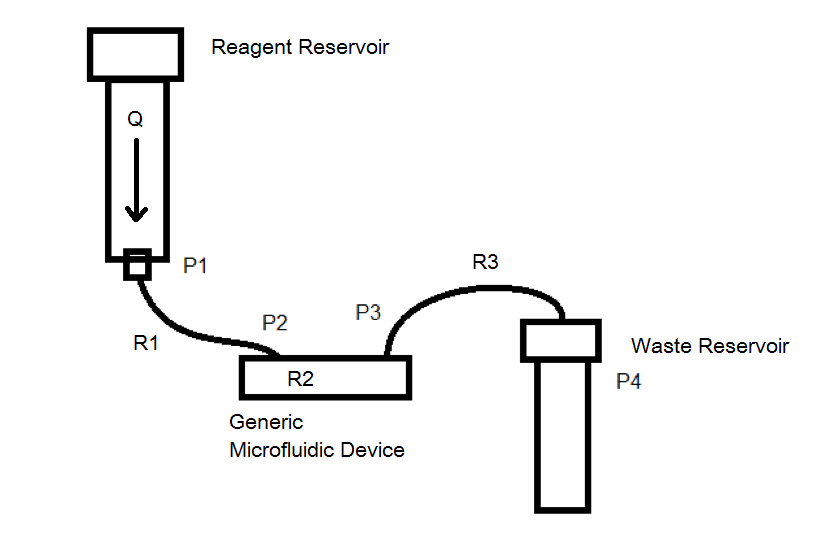
\includegraphics[width=01.0\columnwidth]{resistanceSystem.PNG} 
\caption[Hydraulic Resistance of System]{The microfluidic system detailed from the reagent water column to the waste reservoir.} % The text in the square bracket is the caption for the list of figures while the text in the curly brackets is the figure caption
\label{fig:resistanceSystem} 
\end{figure}

The fluidic resistance due to the reagent reservoirs and tubing leading to the microfluidic device contribute to overall system resistance, and therefore flowrate. However, if the reservoir and tubing widths are substantially larger than the microfluidic device's channels the resistance and therefore contribution to system's pressure loss may be neglected.

For the purpose of quantifying the contribution to total pressure loss of tubing in a generic system the following arbitrary values are applied: Assume that $P_4$ is equivalent to atmospheric pressure, 0 Pa, and $L_1=L_3= 0.500 \ m$, $L_2=0.010 \ m$, viscosity $n=1 \ cP = 0.001 \ Pa \ s$, tube radius$r=0.00025 \ m$ and channel height $h=0.00005m$. Take $P_1 = 500 \ mbar = 50 \ kPa$ which is mid operational range for the system.

Consider the simple case shown in Figure \vref{fig:resistanceSystem}, and that hydraulic resistances in straight circular and square channels can be approximated as shown in Equations \vref{eq:resCirc} and \vref{eq:resSquare}, respectively \cite{Bruus2008}.

\begin{equation}
R_1 = R_3 = \frac{8 \eta L}{\pi r^4}= \frac{8 (0.001) (0.500)}{\pi 0.00025^4} = 3.26  \times 10^7 \frac{kg}{m^4s}
\label{eq:resCirc}
\end{equation}

\begin{equation}
R_2 = \frac{28.4 \eta L}{ h^4}= \frac{28.4 (0.001) (0.010)}{ 0.00005^4} = 4.54 \times 10^{13}\frac{kg}{m^4s}
\label{eq:resSquare}
\end{equation}


Clearly the resistance seen over the length of the simplified microfluidic device of cross-section $50 \mu m \times 50 \mu m$ is several orders of magnitude greater than the resistance of the system's input and output tubing. The flowrate can be calculated as shown in \vref{eq:resFlow}.

\begin{equation*}
P_4 - P_1 = (R_1 + R_2 + R_3) Q
\end{equation*}

\begin{equation*}
Q = \frac{P_4 - P_1 }{(R_1 + R_2 + R3)}
\end{equation*}

\begin{equation}
Q = \frac{50,000}{(2 (3.26*10^7) + 4.54*10^{13})} = 1.10  \times 10^{-9} \frac{m^3}{s} = 1.10  \times 10^{-6} \frac{L}{s}
\label{eq:resFlow}
\end{equation}

Assuming that the system is at steady state and therefore the microfluidic structure (tubing and PDMS) is not expanding due to internal pressure we can infer that by conservation of mass and assumed incompressible fluids that the volumetric flowrate is constant across each of the system pressure points shown in Figure ~\vref{fig:resistanceSystem}. Taking this constant flowrate and the previously found resistances individual pressure drops can be calculated as shown in Equation \vref{eq:resPress}.

\begin{equation*}
P_2 - P_1 = (R_1) Q = 3.59 \times 10^{-2} Pa
\end{equation*}
\begin{equation*}
P_3- P_2 = (R_2)Q = 4.99 \times 10^{4 }Pa
\end{equation*}
\begin{equation}
P_4 - P_3 = (R_3) Q = 3.59 \times 10^{-2} Pa
\label{eq:resPress}
\end{equation}

In this simplified case, representative of a typical microfluidic experimental set-up, the pressure loss due to the tubing relative to the total pressure drop can be calculated as shown in Equation \vref{eq:totalLoss}
\begin{equation}
\frac{(P_2-P_1)+(P_4-P_3)}{P_4-P_1} = \frac{3.59 \times 10^{-2}}{50.00 \times 10^{3}} = 7.18 \times 10^{-7}
\label{eq:totalLoss}
\end{equation}

As the contribution to pressure loss is so small $(<< 1 \%)$, it may be appropriate to neglect the tubing and assume that the PDFC applied pressure is equivalent to the pressure applied across the microfluidic device. This allows the device's pressures to be simplified as shown in Figure \vref{fig:pressureBalance}. The local pressures at the T-junction can then be estimated using the Hagan-Poiseuille law if the channel resistance and flowrates are known.

\begin{figure}[H]
\centering 
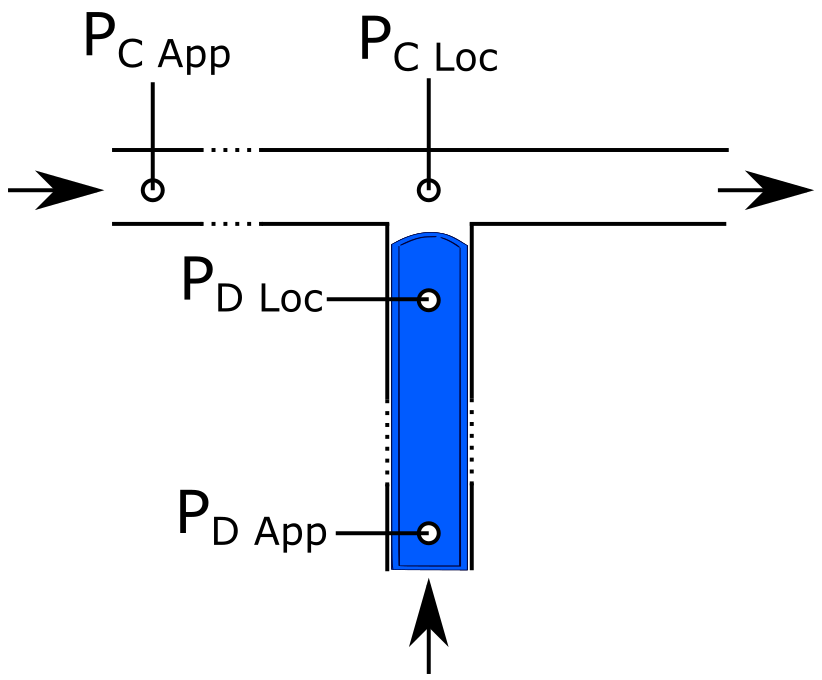
\includegraphics[width=0.75\columnwidth]{pressureBalance.PNG} 
\caption[Pressure Balance at no-flow condition.]{Pressure balance at no-flow condition, where $P_{C App}$ and $P_{D App}$ are the pressures applied to the continuous and discontinuous phases and $P_{C Loc}$ and $P_{D ALoc}$ are the local pressures at the T-junction. The dashed lines represent the channel geometry present between the device inlets and the T-junction.} 
\label{fig:pressureBalance} 
\end{figure}

